% !TeX encoding = UTF-8
% !TeX spellcheck = en_US
% !TeX root = report1.tex


\documentclass[conference]{IEEEtran}
\usepackage{blindtext, graphicx}
\usepackage{amsmath, amsthm, amssymb, amsfonts, nicefrac}



\begin{document}

\title{Monte Carlo Integration and Variational Quantum Mechanics}


\author{\IEEEauthorblockN{Eduardo Villase\~nor}
\IEEEauthorblockA{TU Delft (4624548)}
\and
\IEEEauthorblockN{Ren\'e Vollmer}
\IEEEauthorblockA{TU Delft (4630807)}
\and
\IEEEauthorblockN{Robbie Elbertse}
\IEEEauthorblockA{TU Delft (4078039)}}


\maketitle


\begin{abstract}

Monte Carlo simulations in combination with the variational method is a powerful tool for numerically finding ground states of quantum systems that don't have an analytic solution. In this work we examine and implement this method to approximate the ground states and the associated energies for a one-dimensional harmonic oscillator, a Hydrogen atom and a Helium atom. In order to achieve that goal, different numerical integration methods are examined. In the case of the harmonic oscillator and the hydrogen atom, relative errors in energy smaller than $10^{-5}$ could easily be obtained. For helium much larger errors were observed, since the inter-electron interaction was only approximated with a very simple test-function. Still, the results show that our implementation of the Monte Carlo methods can produce results that are comparable to other methods, even for multi-electron systems.


\end{abstract}

\IEEEpeerreviewmaketitle



% !TeX encoding = UTF-8
% !TeX spellcheck = en_US
% !TeX root = report1.tex


\section{Introduction}
One of the greater problems when dealing with Quantum Mechanics is the lack for a analytical solutions for wave-functions
in almost all cases, where the harmonic oscillator and Hydrogen atom are the most notable exceptions.
Thus different number of numerical methods have been established in order to solve this type
of problem. One of these is the Variational Mont\'e Carlo method, which combines Mont\'e Carlo integration and variational
quantum mechanics in order to solve problems.


\subsection{Mont\'e Carlo Integration: Random Sampling}
\label{ch:monte}
While essentially done through means of computers, there is an 18\textsuperscript{th} century precursor to
his which nicely illustrates the idea of Mont\'e Carlo simulation. In 1733, Georges-Louis Leclerc
de Buffon had a wooden floor made up parallel beams; thus creating a plane with parallel lines.
If we were to drop down needles on the floor, he wondered what the probability would be of
any needle crossing one of the parallel lines \cite{Buffon}. Since this is dependent on the
angle the needle makes with these lines, it comes to no surprise there this is a factor of pi
in the probability. While his intentions were not to find the value of pi, this experiment
was later done to indeed find the value of pi, in 1901 by Mario Lazzarini where after 3408
tosses he found the value of pi up to 7 digits \cite{Lazzarini}.


As of the 1930s the method started to gain more popularity, especially with the advent of the computer. It comes down to using a stochastic method to determine a non-stochastic value.
In the determination of integrals with no known analytical solution, the value of the function can be calculated in a set of points and multiplied with an according area. A sum over a large number of these points can be used to obtain a good approximation of the integral. In order to minimize the computational time, it is desirable, that the number of these points is as small as possible. To still obtain good results, great care must be taken in the choice of the same. We could, for example, imagine, that an equidistant mesh could provide poor results for a cosine function, if the distance between the points has a relation with the period. When dealing with any integral its impossible to always know this in advance,
and so random sample will often provide more accurate results. Purely random points will often form clusters, which will reveal little information. Thus it appears, that starting from a grid and then moving the points a little from their original position constitutes a better strategy. This process of random shifting is called \textit{stratification} of the grid. Additionally, one can divide the space into small subspaces and, after roughly estimating the absolute value of the function in that area, adapt the number of points in that region to the value of the function. Thus areas that contribute in a more significant way to the whole integral, will have a larger number of sample points \cite{MCmethods}.

In this work we explore this idea by comparing different integration methods and observing how taking a large amount of points in a regular grid is not sufficient, and how stratification and adaptiveness in sampling can be utilized to obtain more accurate results.

\subsection{Variational Quantum Mechanics}
The variational method consists at looking at the Hilbert space of a Hamiltonian which contains all the possible wave functions,
that exist in accordance to that Hamiltonian. We then restrict ourselves to a subset of this space,
and try to optimize our solution; for example by finding the ground state energy. The restriction we take is that
we use so-called trial wave functions, which are wave functions of a predetermined format with some unknown parameter(s).
We then attempt to optimize the solution in this parameter space. It turns out that \textit{the} ground state wave function
will always yield the lowest ground state energy. So when comparing two trial wave functions, the one with the lowest
energy will be closer to the \textit{actual} ground state wave function. In this way we can approximate the ground state
energy \cite{AdvStatMech}.


Our goal is to find the ground state and the associated energy of a quantum system. To this end we will
use trial wave functions $\psi_T(\textbf{r},\alpha)$, which is dependent on position(s) $\textbf{r}$ and some variational parameter $\alpha$.
Notice that it is not dependent on time; we are merely interested in the ground state energy and that does not evolve over time.
In order to find the expectation value of the ground state energy we use the equation:
\begin{equation}
	\label{eq:groundstate}
	E(\alpha) = \frac{\int d\textbf{r} \psi_T^*(\textbf{r},\alpha)H\psi_T(\textbf{r},\alpha)}{\int d\textbf{r}
	 \psi_T^*(\textbf{r},\alpha)\psi_T(\textbf{r},\alpha)} \text{~,}
\end{equation}
where $H$ is the Hamiltonian and $E(\alpha) \geq E_0$ is the approximation of the ground state energy, which is always higher
than or equal to the actual ground state energy $E_0$.  We will also define the \textit{local energy}
\begin{align}
	\label{eq:local_energy}
	E_L = \frac{H\psi_T(\textbf{r},\alpha)}{\psi_T(\textbf{r},\alpha)} \text{~.}
\end{align}
%which is a flat function in case that $\psi_T(\textbf{r},\alpha) = \psi_0(\textbf{r})$. By evaluating the variance of $E_L$, we can approximate how far from the ground state energy we are. If the variance is equal to zero we have found an exact solution.
We can make use this local energy, by simplifying equation \ref{eq:groundstate} to:
\begin{equation}
	\label{eq:groundstate2}
	E(\alpha) = \frac{\int d\textbf{r} \psi_T^*(\textbf{r},\alpha)\psi_T(\textbf{r},\alpha)E_L(\textbf{r},\alpha)}{\int d\textbf{r} \psi_T^*(\textbf{r},\alpha)\psi_T(\textbf{r},\alpha)}
\end{equation}
which is easier to work with due to the lack of a Hamiltonian \cite{JosBook}. These integrals can then be numerically evaluated using
the described Mont\'e Carlo method.


%In order to make the best use of finite integration steps, we will sample not \textit{entirely} at random, but rather by iteratively in such a way that we place our finite sample points there where the wave function is non-zero. This is called an adaptive method, and we will show that this yields better results quicker than using an entirely random sample, as seen in the next chapter.
%In order to calculate the variance of the local energy, we take
%$Var(E_L) = \sqrt{<E_L^2> - <E_L>^2} = \sqrt{ \int \textbf{r}^2 E_L(\textit{r},\alpha) d\textbf{r} - (\int \textbf{r} E_L(\textit{r},\alpha)d\textbf{r})^2 } $, %TODO!!!
%which can either be solves analytically or numerically, depending on the form of the local energy.

The goal is, to find the minimum value of the energy with respect to $\alpha$. The direct derivative $\frac{dE}{d\alpha}$ can unfortunately be misleading, since fluctuations in the energy values due to integration errors can be larger than the actual gradient. Thus Newton's method on the derivative is utilized to write
$$\frac{dE}{d\alpha} = 2 \left( \left< E_L \frac{d \ln(\Psi_T)}{d \alpha} \right> - E\left<\frac{d \ln(\Psi_T)}{d \alpha}\right> \right) \text{~.}$$
This method works because our the exact solution is within the family of trial functions, see \cite{JosBook}. %TODO
The new variational parameter can then recursively be adapted with $$\alpha_{\text{new}} = \alpha_{\text{old}} - \gamma \frac{dE}{d\alpha} \text{~} $$
to find the minimum of the energy with respect to alpha.



%TODO: Not sure if this is appropriate in a paper
%This work is as follows, chapter 2 contains a theoretical description of the quantum problems we attempt to solve. In chapter 3 we explore through different numerical integration methods comparing each other in order to conclude which one is the best. Next in chapter 4, we describe our results and discuss them in the light of expectations. Finally, in chapter 5 we will draw conclusions and suggest options for further research.



\section{Making a Monte Carlo integrator}
\label{ch:monte_app}

First, we explored different methods in order to gain a better insight on how to create a good general integrator. We tested 4 methods, where each differs in how the points in the domain are chosen to evaluate the integral (compare to chapter~\ref{ch:monte}):
\begin{enumerate}
  \item Uniform Static - The entire domain is divided by a uniform mesh were each point is taken in a coordinate is the grid.
  \item Uniform Adaptive - The domain is divided uniformly in square boxes, and for each box a mesh grid is created
  specified by a density value which determines the total number of points inside that box. The density parameter
  is obtained by performing successive iterations, on which the density of each sub-box is set by the total value of the integral inside
  the box.
  \item Stratified Static - The entire domain is divided in a uniform mesh, where for each quadrant of the mesh
  a single point is chosen randomly inside.
  \item Stratified Adaptive - A combination of both methods adaptive and stratified.
\end{enumerate}
\begin{figure*}
  \begin{center}
    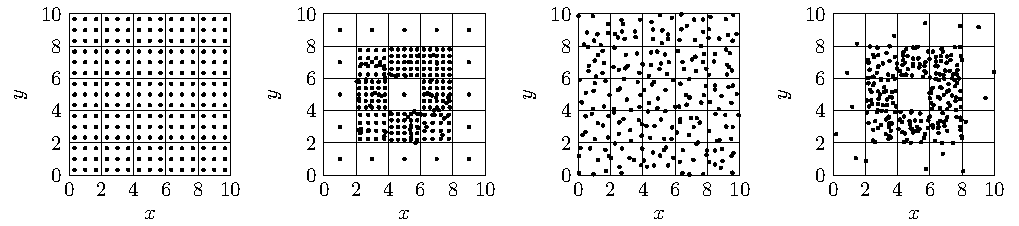
\includegraphics[scale=1 ]{graphs/BoxPlotter.pdf}
  \caption{Illustrative examples of (from left to right) a uniform static, uniform adaptive, stratified static and stratified adaptive integration schemes. The lines create boxes within which an internal grid is applied in the case of static integration schemes. Notice that in all cases the number of points is the same, which in the case of adaptive static causes us to end with some points which do not fit in a grid. To accommodate for this we distributed them randomly within their respective box. }
\label{BoxPlotter}
  \end{center}
\end{figure*}

To compare these methods we used a ring-shaped test function over which we evaluated the integrals. This two-dimensional ring, with an outer radius of 4 and an inner radius of 2, the value is 2, outside it is zero. The analytical integral over the whole domain is thus simply $ A=2\pi (4^2-2^2)$.  In figure~\ref{BoxPlotter} a set of sampling point distributions for this test function and each method are shown. To compare the performance of these methods, each of them were executed at a different number of test points. The obtained results were compared with the analytical answer and over several repetitions the average error determined. These results are shown in fig. \ref{MCerrs}, where 1,000 repetitions where used for each number of points. In the case of adaptive methods the entire integration domain was divided into 25 boxes.

One can clearly see, that only certain number of points can be achieved with the uniform methods, since the points always need to fit in a grid. For the uniform static method no deviation can be seen. This is due to the fact, that this method is fully deterministic and thus all repetitions with the same parameters return the same result.
As expected the best results are obtained with the adaptive stratified method, which has also gives the smallest standard deviation from the error as seen in the error bars (with the exception of the uniform static method).
Additionally it is important to note how the error of the uniform static method, and in lesser degree in the adaptive static, increases at some point as the number of points increases, this systematic error introduced by the regular mesh. This shows the entire point of doing Monte Carlo integration!
\begin{figure*}[ht]
  \begin{center}
  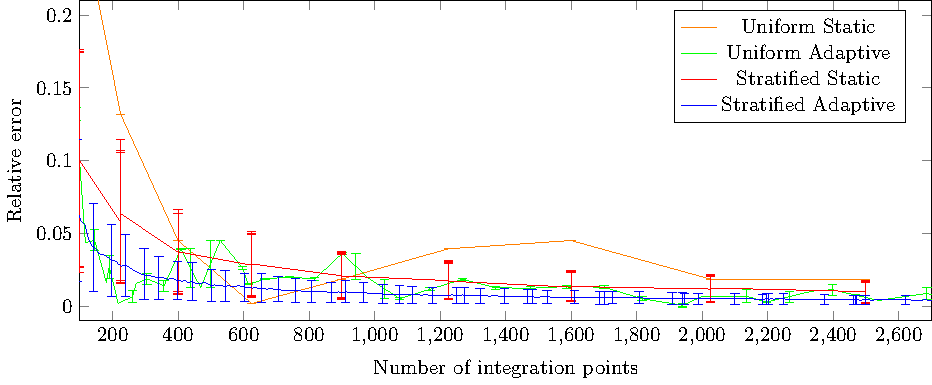
\includegraphics[scale=1 ]{graphs/integration_test_ring.pdf}
  %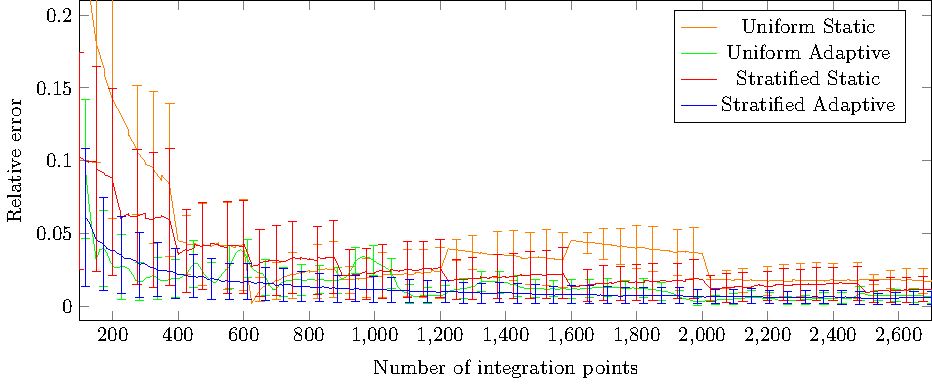
\includegraphics[scale=1 ]{graphs/integration_test_ring_rand.pdf}
  \caption{Performance comparison of different numeric integration methods. The absolute value of the difference between the numerically calculated result and the analytical answer plotted against the number of integration points used. The used function is a two-dimensional ring (see text).}
  \label{MCerrs}
  \end{center}
\end{figure*}


% !TeX encoding = UTF-8
% !TeX spellcheck = en_US
% !TeX root = report1.tex

\section{Variational}
%Now we focus on using the integration to solve the problem established in the introduction.
In this section, we will use the Monte Carlo integration to solve three different problems, the one-dimensional harmonic oscillator, hydrogen atom and helium atom.

\subsection{Harmonic Oscillator}
The Hamiltonian of the harmonic oscillator is
\begin{align*}
	\hat{H} = \frac{-1}{2}\frac{\partial^2}{ \partial x^2} + \frac{1}{2} x^2  \text{~.}
\end{align*}
Where we choose the trial wave function as
\begin{align*}
	\Psi_T = e^{-\alpha x^2} \text{~.}
\end{align*}
With this and eq.~\eqref{eq:local_energy}, we can calculate the local energy:
\begin{align*}
	E_L = \alpha + x^2 \left(\frac{1}{2} - 2\alpha^2\right) \text{~.}
\end{align*}
 	
Notice that, based on the local energy we can already determine that $\alpha = \nicefrac{1}{2}$ gives us the ground state ($E_L = E_0 = \nicefrac{1}{2}$), because in that case the variance of the local energy is equal to zero. It is nonetheless a good test for our algorithm to see if we can find the expected value of $E_0 = \nicefrac{1}{2}$ using Monte Carlo integration.\\
  
We apply the stratified adaptive integration scheme as defined in section~\ref{ch:monte_app} and use Newton's method on the derivative $\frac{dE}{d\alpha} = 2 (\left< E_L \frac{d \ln(\Psi_T)}{d \alpha} \right> - E\left<\frac{d \ln(\Psi_T)}{d \alpha}\right>)$. This method works because our the exact solution is within the family of trial functions, see \cite{JosBook}. %TODO
The new variational parameter can then be adapted as $$\alpha_{\text{new}} = \alpha_{\text{old}} - \gamma \frac{dE}{d\alpha} \text{~.} $$

Two simulations for the one-dimensional harmonic oscillator were performed with 50 iterations, a damping factor of $\gamma = 10^{-5}$, an initial value of $\alpha_i = 3~/~ 0.01$ for alpha and 1,000 test points over a domain with length 4, subdivided into 20 sub-domains for the adaptive grid. With this, we obtained an energy of $E_{MC}-E_0 \simeq 1.63\cdot 10^{-9}$ at $\alpha - \alpha_0 \simeq 7.6455\cdot 10^{-6}$, compare to figure~\ref{fig:Ho_it} and \ref{fig:Ho_rel}. %TODO: Are these numbers correct? Where were they taken from? What is the difference for the two alpha_i's?

\begin{figure}[th]
	\begin{center}
		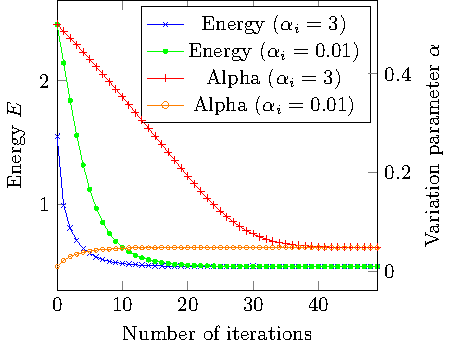
\includegraphics[scale=0.9]{graphs/ho-e-alpha-iterations.pdf}
		\caption{
			Energy and alpha as a function of iteration number. %TODO: Some more caption. Mention Harmonic Osci
			%Calculated $E$ as a function of $\alpha$ using two different starting values for$\alpha_0$. Notice that $\alpha$ converges monotonically (increasing or decreasing) while this is not necessarily true for the energy due to the integration not being exact. Nonetheless, a very accurate result can be found: $E_{\alpha_0 = 0.5} =  $ and $E_{\alpha_0 = 0.5} =  $.
			}
		\label{fig:Ho_it}
	\end{center}
\end{figure}
\begin{figure}[th]
	\begin{center}
		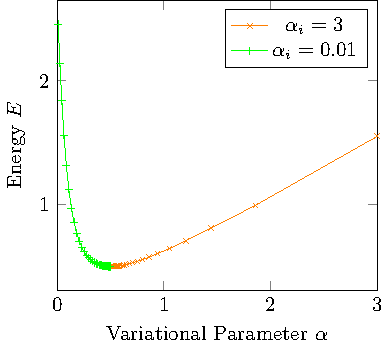
\includegraphics[scale=0.9]{graphs/ho-e-alpha.pdf}
		\caption{
			Energy plotted as a function of alpha. %TODO: Some more caption. Mention  Harmonic Osci
			%Calculated $E$ as a function of $\alpha$ using two different starting values for$\alpha_0$. Notice that $\alpha$ converges monotonically (increasing or decreasing) while this is not necessarily true for the energy due to the integration not being exact. Nonetheless, a very accurate result can be found: $E_{\alpha_0 = 0.5} =  $ and $E_{\alpha_0 = 0.5} =  $.
		}
		\label{fig:Ho_rel}
	\end{center}
\end{figure}
  

\subsection{Hydrogen Atom}
We will now consider the Hydrogen atom, where the Hamiltonian is
\begin{align*}
  \hat{H} = -\frac{1}{2}\nabla^2 - \frac{1}{r} \text{~.}
\end{align*}

We choose the trial wave function as
  \begin{align*}
    \Psi_T = e^{-\alpha r} \text{~,}
  \end{align*}
which leads to the local energy
  \begin{align*}
    E_L(r) = - \frac{1}{r} - \frac{1}{2}\alpha \left(\alpha - \frac{2}{r}\right) \text{~.}
  \end{align*}

Here, too, we notice that from inspection it is clear that $\alpha = 1$ yields the ground state energy of $E_L = E_0 = -\nicefrac{1}{2}$, because there $\text{Var}(E_L) = 0$. The convergence on this seems to be quite fast. Using the parameters $\gamma = 5\cdot 10^{-4}$, $\alpha_i = 3 \text{~/~}0.01$ with 5,000 test points over $7$ boxes, we need about 160 iterations to reach $\alpha-\alpha_0 \simeq 5 \cdot 10^{-10}$. That is, within 160 iterations we can estimate $\alpha$ up to ten digits and find the appropriate energy for it. 


\subsection{Helium Atom}
Finally we consider the Hamiltonian for the Helium atom,
\begin{align*}
  \hat{H} = -\frac{1}{2} \left(\nabla_{r_1}^2 + \nabla_{r_3}^2 + 2\nabla_{r_1}\cdot \nabla_{r_2}\right)  - \frac{1}{r} \text{~.}
\end{align*}
Where will we use the trial function
  \begin{align*}
    \Psi_T (\textbf{r}_1,\textbf{r}_2) = e^{2r_1}e^{2r_2}e^{\frac{r_{12}}{2(1+\alpha r_{12}}}
  \end{align*}

where $r_{12} =  \left|\textbf{r}_1 - \textbf{r}_2 \right| $. This leads a rather simple equation for the local energy:
\begin{align*}
    E_L(\textbf{r}_1,\textbf{r}_2) &= -4  +  \frac{(\hat{\textbf{r}}_1 - \hat{\textbf{r}}_2) (\textbf{r}_1 - \textbf{r}_2)}{r_{12}(1+\alpha r_{12})^2} - \frac{1}{r_{12}(1+\alpha r_{12})^3}  \\
    &~~~ - \frac{1}{r_{12}(4(1+\alpha r_{12}))^4} + \frac{1}{r_{1,2}}
\end{align*}
  
This, too, we solved with using the stratified adaptive integration method, and changing $\alpha$ like we did at the Harmonic Oscillator and the Helium atom. Using two different starting values $\alpha_i$ we convergence to the same values for $\alpha$ and $E_{MC}$, see figure~\ref{fig:He_it}. The values we find for the energy after just 50 iterations are $E_{\alpha_i = 0.01} =  $ and $E_{\alpha_i = 0.5} =  $, which compare well with the optimum value achieved by this method of $-2.8781 \pm 0.0005$, the Hartree-Fock value of $-2.8617$, the DFT value of $-2.83$ and the exact value of $-2.9307$ (see \cite{JosBook}). %TODO

\begin{figure}
  \begin{center}
  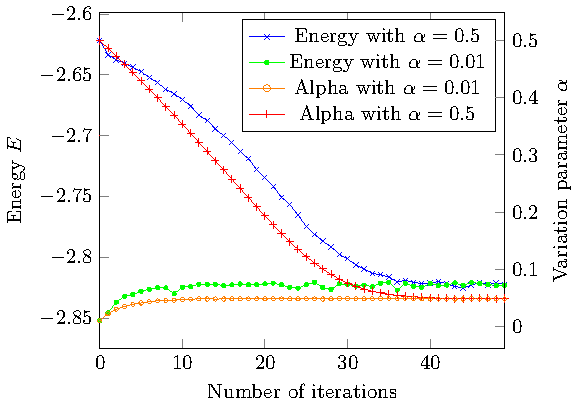
\includegraphics[scale=1 ]{graphs/he-e-alpha-iterations.pdf}
  \caption{
  	Calculated $E$ as a function of $\alpha$ using two different starting values for$\alpha_0$. Notice that $\alpha$ converges monotonically (increasing or decreasing) while this is not necessarily true for the energy due to the integration not being exact. Nonetheless, a very accurate result can be found: $E_{\alpha_0 = 0.5} =  $ and $E_{\alpha_0 = 0.5} =  $
  	%TODO: This was already mentioned in the text. I should only be in one place! Also mention, that this is Helium
  	}
  \label{fig:He_it}
  \end{center}
\end{figure}
 


% !TeX encoding = UTF-8
% !TeX spellcheck = en_US
% !TeX root = report1.tex


\section{Conclusion}
We investigated four different integration schemes and found that although using stochastically chosen points does not \textit{necessarily} give better results, the relative error decreases monotonically as a function of integration points. This property is very valuable when trying to minimize the error in your calculations. Furthermore, we found that adaptively changing the probability distribution of data points gives yields better results over taking treating all space equal. The combination of both, the stratified adaptive method seems to dominate in its usefulness. \\

Furthermore we found that we can easily calculate the ground state energy with a relative error in the order of $10^{-9}$ using trial functions, in the case of the harmonic oscillator and the hydrogen atom. For the helium atom we found a relative error of <INSERT OUR VALUE DIVIDED BY -2.9307> which is similar to that of other methods such as Hertree-Fock and DFT calculations. Part of the reason that we are this much off is because the actual eigenfunction is not within our family of trial functions. Unfortunately this eigenfunction is not known and so we cannot purposefully propose a family of trial functions which contains it. Nonetheless, our results are in line with different methods and so we may conclude that our method succeeds, especially since it does not require a lot of computing power. \\

For future research it will be interesting to investigate possible improvements to the stratified adaptive method. For example, we now used boxes to adapt to our probability distribution, but perhaps other geometries are more efficient (concentric rings when $\Psi_T = \Psi_T(r)$, or triangles akin to finite element methods). It is also interesting to investigate other Hamiltonians, including those whose eigenfunctions are not known analytically. 














\bibliographystyle{plain}
\bibliography{report}


\end{document}
